%%%%%%%% ICML 2021 EXAMPLE LATEX SUBMISSION FILE %%%%%%%%%%%%%%%%%

\documentclass{article}

% Recommended, but optional, packages for figures and better typesetting:
\usepackage{microtype}
\usepackage{graphicx}
\usepackage{float}
\usepackage{subfigure}
\usepackage{booktabs} % for professional tables
\usepackage{amssymb}
% hyperref makes hyperlinks in the resulting PDF.
% If your build breaks (sometimes temporarily if a hyperlink spans a page)
% please comment out the following usepackage line and replace
% \usepackage{icml2021} with \usepackage[nohyperref]{icml2021} above.
\usepackage{hyperref}

% Attempt to make hyperref and algorithmic work together better:
\newcommand{\theHalgorithm}{\arabic{algorithm}}

% Use the following line for the initial blind version submitted for review:
% \usepackage{icml2021}

% If accepted, instead use the following line for the camera-ready submission:
\usepackage[accepted]{icml2021}

% The \icmltitle you define below is probably too long as a header.
% Therefore, a short form for the running title is supplied here:
\icmltitlerunning{}

\begin{document}

\twocolumn[
\icmltitle{Data Augmentation as an Inverse Problem}

% It is OKAY to include author information, even for blind
% submissions: the style file will automatically remove it for you
% unless you've provided the [accepted] option to the icml2021
% package.

% List of affiliations: The first argument should be a (short)
% identifier you will use later to specify author affiliations
% Academic affiliations should list Department, University, City, Region, Country
% Industry affiliations should list Company, City, Region, Country

% You can specify symbols, otherwise they are numbered in order.
% Ideally, you should not use this facility. Affiliations will be numbered
% in order of appearance and this is the preferred way.
\icmlsetsymbol{equal}{*}

\begin{icmlauthorlist}
\icmlauthor{Hayden Prairie}{}
\icmlauthor{Frank Collebrusco}{}
\icmlauthor{David Shilliday}{}
\icmlauthor{Ranit Gupta}{}
\icmlauthor{Ashwin Ram}{}
\icmlauthor{Andrew Wang}{}
\end{icmlauthorlist}

\icmlcorrespondingauthor{Hayden Prairie}{haydenprairie@utexas.edu}

% You may provide any keywords that you
% find helpful for describing your paper; these are used to populate
% the "keywords" metadata in the PDF but will not be shown in the document

\vskip 0.3in
]

% this must go after the closing bracket ] following \twocolumn[ ...

% This command actually creates the footnote in the first column
% listing the affiliations and the copyright notice.
% The command takes one argument, which is text to display at the start of the footnote.
% The \icmlEqualContribution command is standard text for equal contribution.
% Remove it (just {}) if you do not need this facility.

% \printAffiliationsAndNotice{}  % leave blank if no need to mention equal contribution
% \printAffiliationsAndNotice{\icmlEqualContribution} % otherwise use the standard text.

\begin{abstract}
With the growth in the complexity of neural networks and the amount of available compute, the need for larger datasets
has become a bottleneck in the advancements of computer visions. In this paper we explore an new approach to synthetic
data generation by treating data augmentation as an inverse problem. We ultize posterior sampling with latent diffusion
models in order to generate synthetic data through masking. Finally we discuss potential improvements and future work
that can be done. Code is available at \url{https://github.com/Hprairie/Synthetic-ImgGen-PSLD}.
\end{abstract}

\section{Introduction}
\label{introdcution}

In recent years deep learning has made incredible strides in computer vision tasks such as image classification,
object detection, and semantic segmentation. Most advancements within this feild can be attributed to the improvement
of novel architectures, an increase in compute, and access to large datasets. However, the ability to scale a model
without scaling the size of its correspondeing dataset has been show to have diminishing returns \cite{2001.08361}.
The ability to generated large labeled datasets by hand is infeasable and thus the need for unsupervised techniques to create
augmented or synthetic data become's necissary. Niave approaches to data augmentation such as random cropping, flipping,
rotation, etc. have been shown to be effective in some cases, but unfeasable in other cases such as medical imaging, where
niave approaches create unrealistic image domains. More advanced techniques such as generative adversarial networks
\cite{1406.2661} have been shown to be effictive in creating realistic synthetic data, however these often require large amounts of data in
order to fine tune models.

In the last year the surge in the power of large language models such as GPT-4 has also shown their potential to create synthetic
data \cite{2304.13861}. The ability for LLMS to generate realistic text responses to prompts could be viewed as an inverse problem, in which the LLM is attempting
to find the most likely text given a prompt. A similar approach can be taken with images, where diffusion models can be used to solve
inverse problems and in turn generate synthetic data.

In this paper we explore the use of posterior sampling with latent diffusion models (PSLD) \cite{rout2023solving} to create synthetic data. PSLD
allows the us to leverage the power of latent diffusion models in order to solve linear inverse problems in images. By
generating a mask and then using PSLD to reconstruct the image, variations of the original image can be created,
due mainly the inherent lossy relations of masking pixels. We found these synthetic images to be effective in improving
the performance of object detections models.

The rest of the paper is organized as follows. First we cover the related work along with the benefits and downsides of niave and advanced data
augmentation techniques. Then we cover our approach of treating augmentation as an inverse problem and utilize diffusion
models for synthetic data generation. Finally we cover the results of our initial expirements and potential improvements along
with future work that can be done.
 

\section{Related Work}

Data Augementation and synthetic data generation aim to artifically increase the size of training set in order to improve robustness
of computer vision models and prevent overfitting to a training set. Similar to dropout in neural networks, data augmentation can be
useful in leading a model to a more generalizable solution \cite{1708.04896}.

\subsection{Niave Data Augmentation}

Most niave data augmentation techniques apply simple tranformations to the input image while maintaining the label, such as flipping,
cropping, rotating, translation, color jittering, and adding noise. Other more complex techniques such as random erasing aim to occlude
parts of the image allowing the model to learn to focus on other features. These techniques are often effective in improving the performance
of image classification models, however they are often negligble in object detection settings \cite{2204.08610}. Furthermore these trasnformations are often ignorant 
to certain domains such as medical imaging, where simple transoformations are not applicable to potential real world domains.

For example in brain ct scans, linear transformations of the image would create unrealistic domains that are not representative of test/validation data. 
The use of linear transformations in order to improve the robustness of a model in these domains often doesn't work as infrence time samples will be centered 
and cropped such as in ct scans. Thus the need for variation in the training set under specific domain constraints are necissary. 

\subsection{Advanced Data Augmentation}

In more recents years the use of generative adversial networks (GANS) \cite{1406.2661} have been show to be effective in creating realistic images. Several papers
have attempted to leverage their power to create synthetic \cite{1911.02888}, \cite{2104.06490}, \cite{2106.05258}. While the techniques have been seen to be effective,
their ability to generate realistic images pales in comparison to latent diffusion models \cite{2112.10752}. Especially when considering the the power of latent diffusion
once trained on datasets as LAOIN-5B \cite{2210.08402}, the power of GANs is pale in compraison.

\subsection{Diffusion Models}

As the power of latent diffusion models grows, the desire to apply their power to synthetic data generation has become increasingly more popular. Some work
attempts to graft target images partway through the diffusion process creating more variations of the original images at the cost of faithfulness to the target
class \cite{2108.01073}. This was then tested in zero shot and few shot settings, where it was shown to be effective in improving the performance of image 
classification \cite{2210.07574}. In both of these situations the diffusion model is guided by the text prompt, creating another issue as the model is unable to
generalize to new images where vocabulary is used outside of its training set. Other work has attempted to solve this by insert embeddings into the textual encoder
and then using textual inversion to fine tune the model, allowing it to generalize new vocabulary \cite{2302.07944}. However the significant issue with these approaches
is their higher likelihood to generate unfailful images and their need to fintune the diffusion model, which often requires a large amount of compute.

There is some work on the use of inpainting in semantic segmentation tasks, where morphological erosion was applied to the mask which allowed the model to better
generalize the inpainting process and inpaint more faithfull images \cite{Pobitzer_2023}. However there are still some issues with this approach as well,
as the model is still uses prompt guidance and is unable to generalize to new domains not in its training vocabulary.

\section{Our Approach}

A desirable way to create synthetic data would create more variation than niave data augmentation techniques, but without the need for
large data and compute to train GANs. Thus we propose a method of treating data augmentation as an inverse problem, in which synthetic samples
can be generated by utilizing PSLD and allowing the latent diffusion models to fill in missing pixels. For example, consider the matrix $A$ which
transforms the image $x$ to 'corrupted' image $\hat{x}$ and can then be passed to the PSLD algorithm which will attempt to reconstruct
the original image $x$. The resulting image is a synthetic sample $\tilde{x}$ which can be then be used as a training sample. In this paper we
only attempt to reconstruct an image through masking, however other transformations such as gaussion blurring, motion blurring, and lossy compression
could potentially be used as well.

\begin{figure}[ht]
    \vskip -0.1in
    \begin{center}
        \centerline{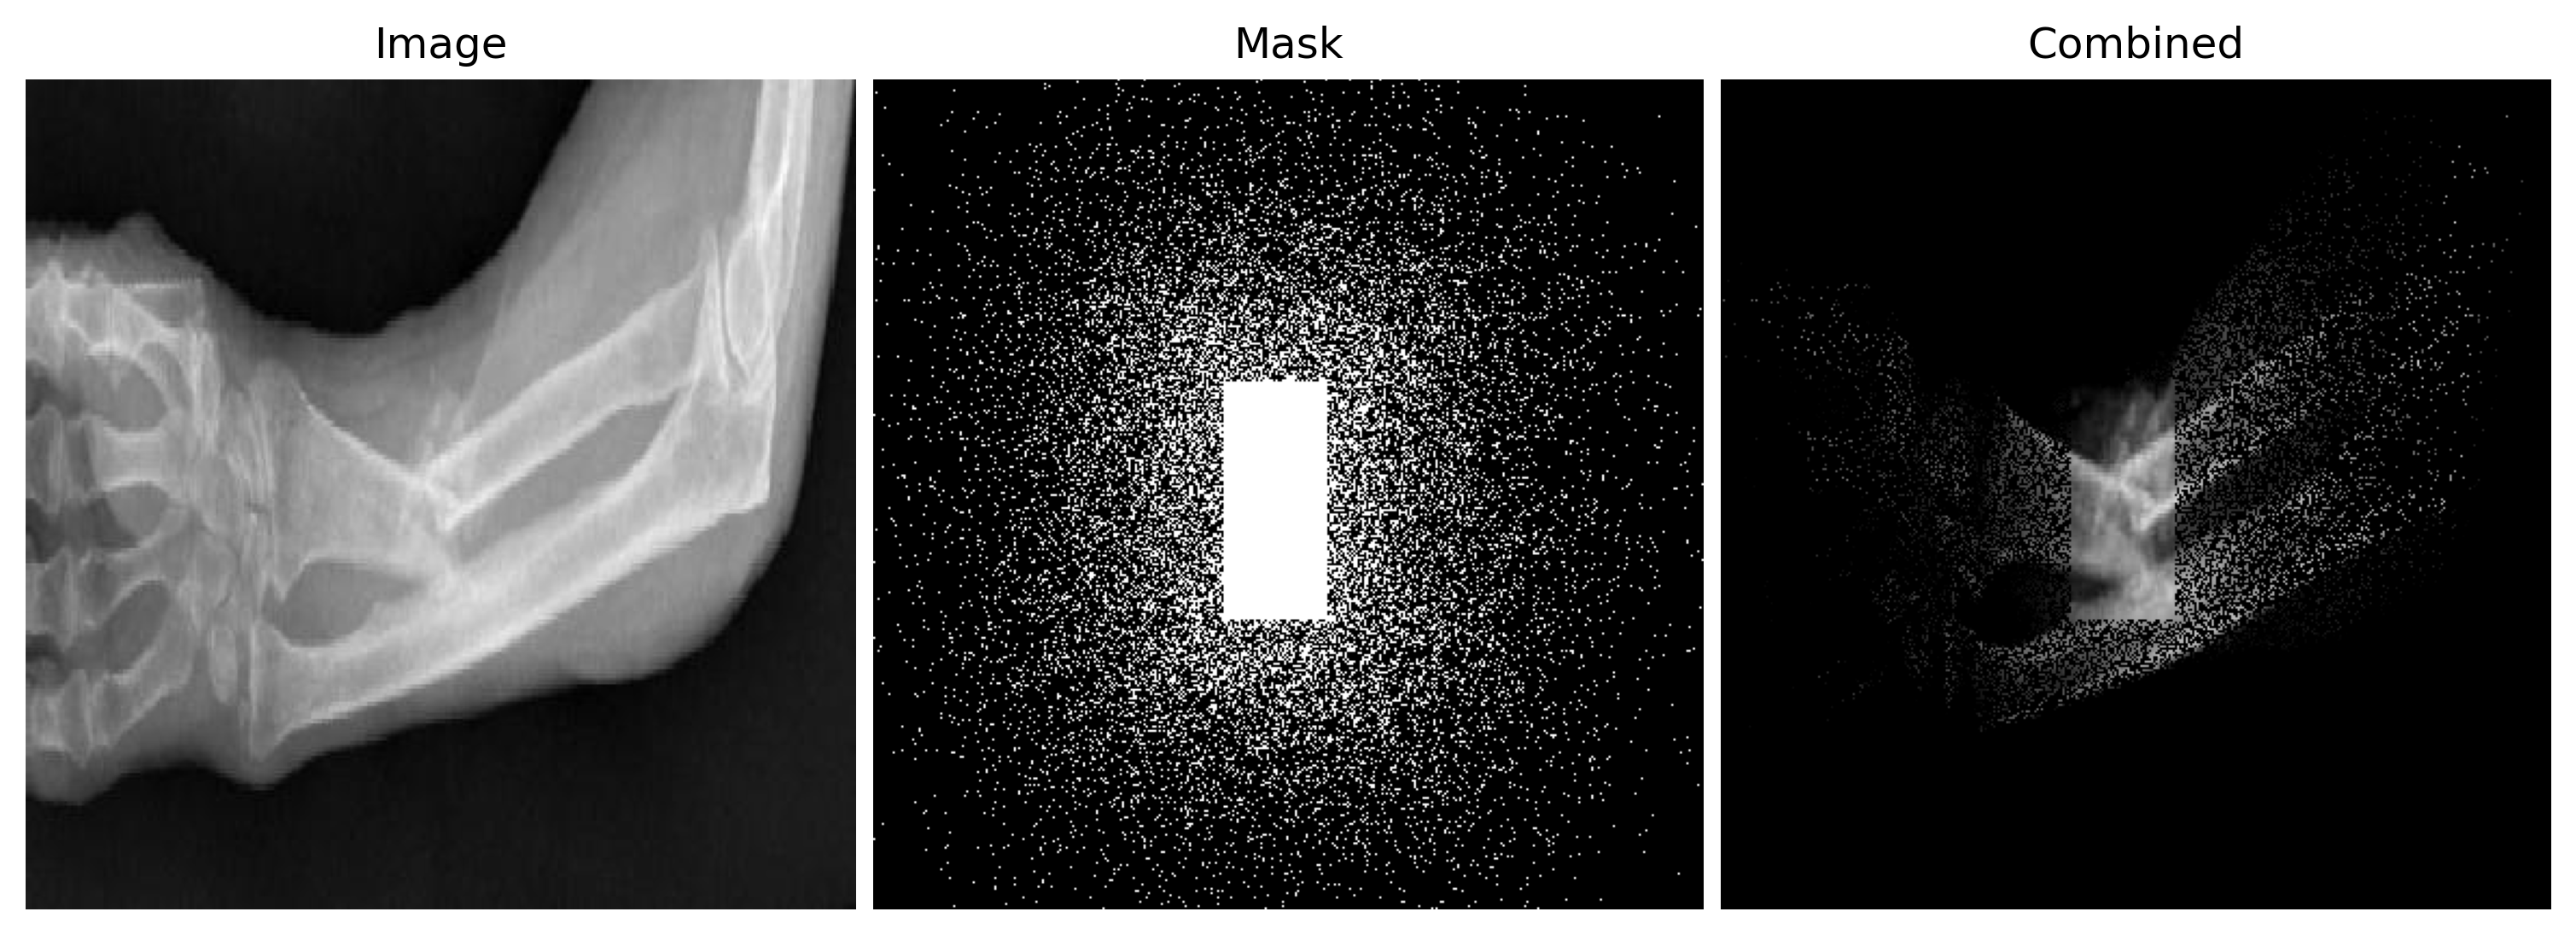
\includegraphics[width=\columnwidth]{Mask.png}}
        \caption{Example of sample passed into stable diffusion with corresponding image and mask.}
        \label{psld_mask}
    \end{center}
    \vskip -0.3in
\end{figure}

While several masking techniques could potentially be useful, i.e. random, gaussian, in bounding box, out of bounding box, etc. we only tested on
gaussian out of the bounding box masking, which is displayed in Figure \ref{psld_mask}. A mask can be generated by first completely masking the inside 
of a given samples bounding box and then creating 
a matrix $D$ which is the same shape of our image but contains the distance from any given pixel to the nearest masked pixel. We can then sample a gaussian
distribution $N \sim (0, \sigma)$ at each pixel, and then mask any pixel where $d \in D$ is greater than it's given sample from $N$. This results in a mask where pixels
closer to the bounding box are more likely be masked than pixels further away from the bounding box. 

\begin{figure}[ht]
    \vskip -0.1in
    \begin{center}
        \centerline{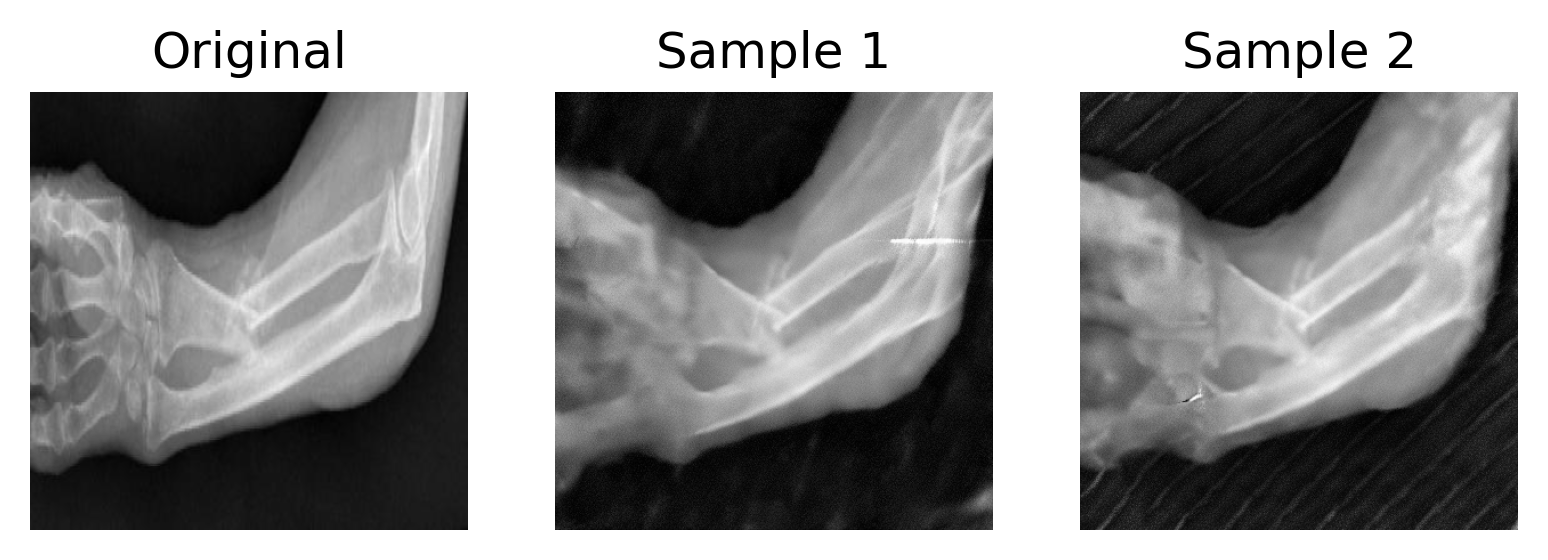
\includegraphics[width=\columnwidth]{psld_results.png}}
        \caption{Example of sample passed into stable diffusion with corresponding image and mask.}
        \label{psld_results}
    \end{center}
    \vskip -0.3in
\end{figure}


\begin{table*}[ht!]
\centering
\caption{Your caption}
\label{results}
\begin{tabular}{lcccccr}
\toprule
Augmentation & Train Box $\downarrow$ & Train Objective $\downarrow$ & Val mAP@0.5 $\uparrow$ & Val F1  $\uparrow$ & Test mAP@0.5 $\uparrow$ & Test F1 $\uparrow$\\
\midrule
Baseline & 0.02726 & 0.004067 & 0.6969 & 0.73 & 0.699 & 0.73\\
Naive &  0.03984 & 0.005202 & 0.7298 & 0.74 & 0.746 & 0.73\\
PSLD & \textbf{0.0254} & \textbf{0.003194} & \textbf{.7349} &  \textbf{0.77} & \textbf{0.782} & \textbf{0.82} \\
\bottomrule
\end{tabular}
\end{table*}

The image with it's corresponding mask can then be \textit{solved} as an inverse problem using the PSLD algorithm, creating new synthetic samples due to the lossy nature
of estimating pixel values. Examples of resulting images can be seen in Figure \ref{psld_results}.

As described this approach allows the creation of synthetic samples samples that are not prompt guided or limited to a given vocabulary, don't require model
finetuning, and are not limited to a given domain. However, the downside to this approach is that realism in the generated images, as a preference to class faithfulness
comes at the cost of realism.



\section{Experiment}

We ran several experiments on the effectiveness of synthetic data generation using PSLD. We used a bone fragment dataset which consists of 1000 images 
(750 train, 50 val, 200 test) of bone fractures from all over the body \cite{bone-fracture-detection-ivsy6_dataset}. The reasoning for using this dataset is 
it's increased probability of lying outside the training set. We used stable diffusion v1.4 \cite{Rombach_2022_CVPR}, a latent diffusion model trained on 
LAION-Aesthetics V2 \cite{2210.08402}. We created roughly 1000 synthetic samples using PSLD, and then compared it with other naive data augmentation techniques 
where we created a similar number of samples.

\begin{figure}[ht]
    \vskip -0.1in
    \begin{center}
        \centerline{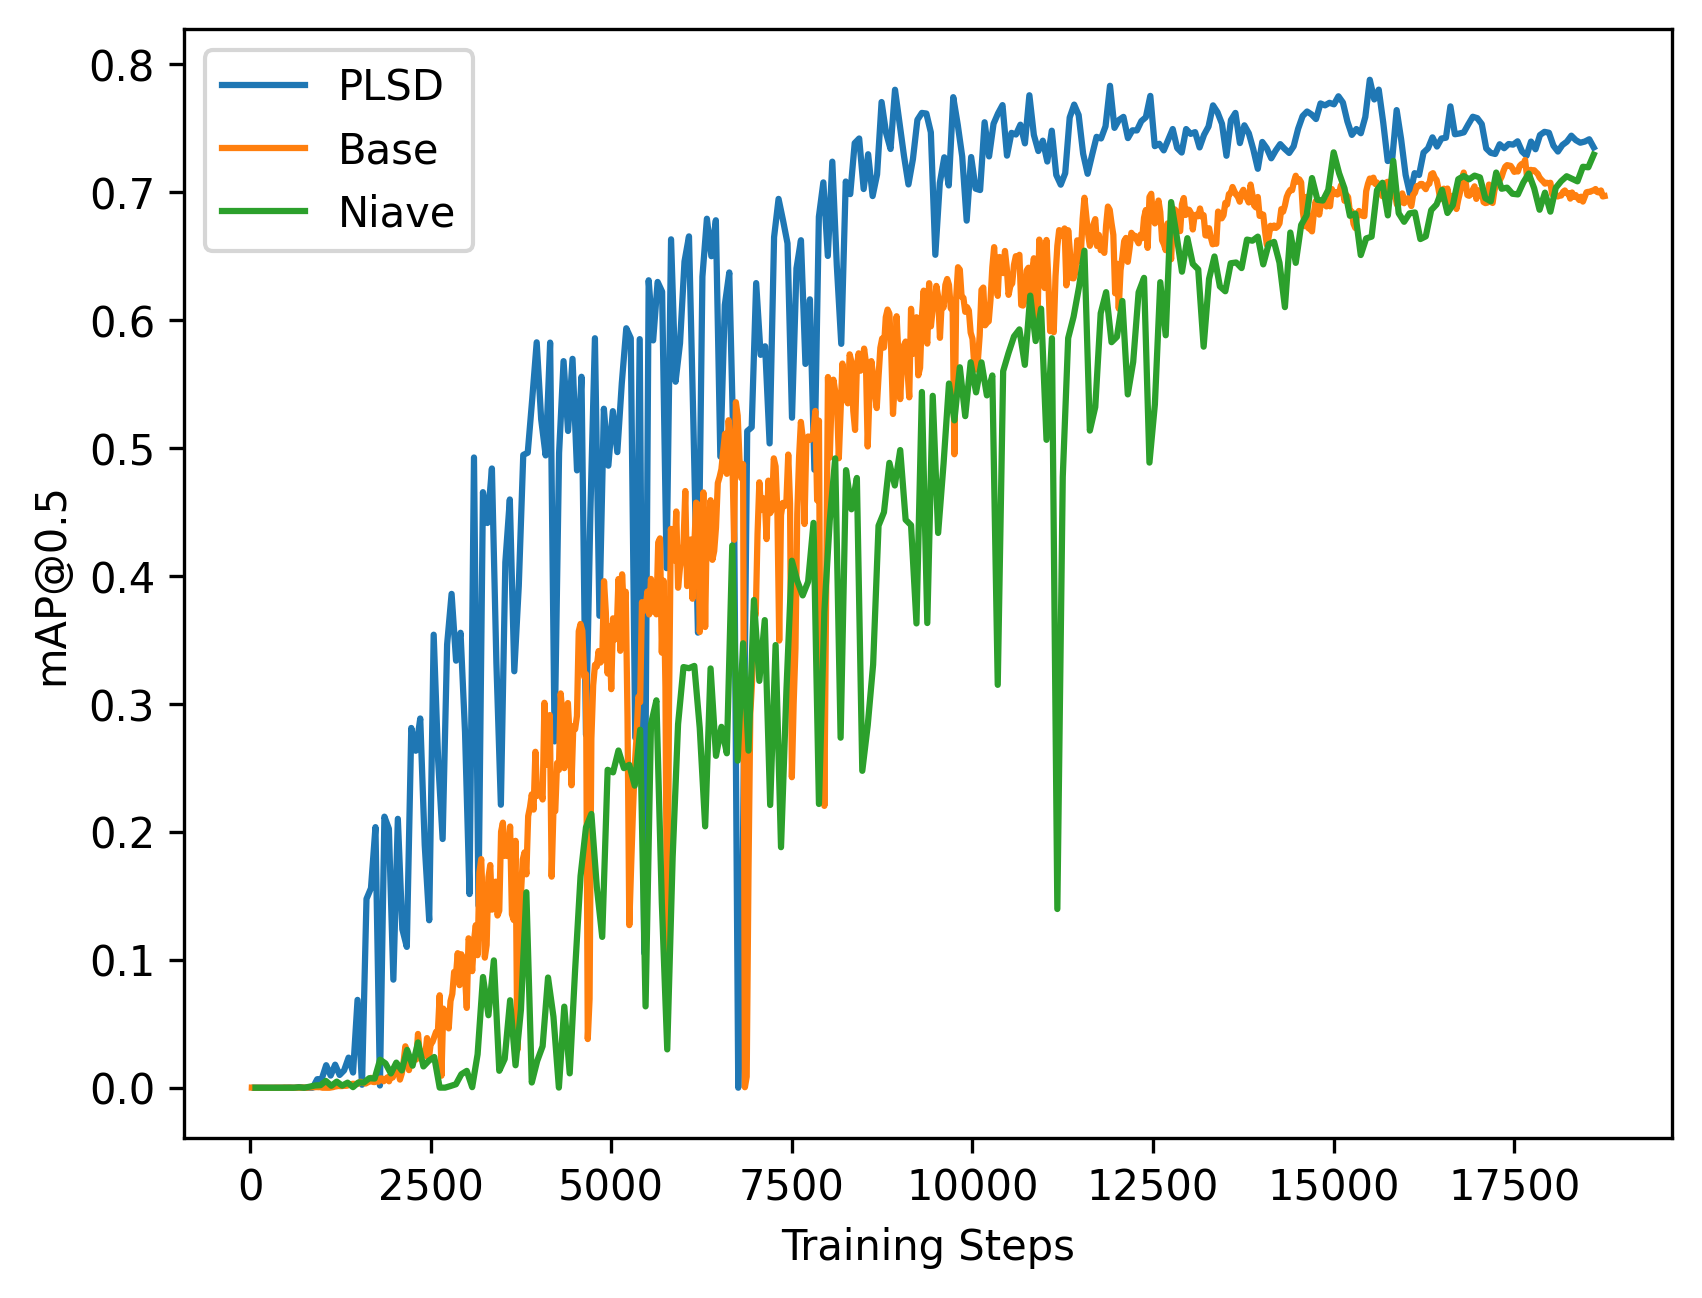
\includegraphics[width=\columnwidth]{training.png}}
        \caption{Training curves of YOLOv7 model with respect to each data type.}
        \label{training_curves}
    \end{center}
    \vskip -0.3in
\end{figure}


The results of the experiment can be seen in Table \ref{results} where we compare the performance of a YOLOv7 model \cite{wang2023yolov7}. We found that 
the use of synthetic data was incredibly effective in improving the performance of our baseline YOLOv7 model. Compared with other naive data augmentation techniques,
we found that the use of PSLD was also more effective in improving the performance of our model. The training curves of the model can be seen in 
Figure \ref{training_curves}, which is adjusted for gradient steps instead of epochs.

One thing interesting to note is that samples are often to visually different, however there is often large differences at the pixel level.
This can be seen in Figure \ref{difference}, where the difference between the two images at a pixel level is shown scaled to an extremely large exponent of 400.
Nevertheless, this still enables to model to learn more robust features and generalize to the validation and test set.


\begin{figure}[ht]
    \vskip -0.1in
    \begin{center}
        \centerline{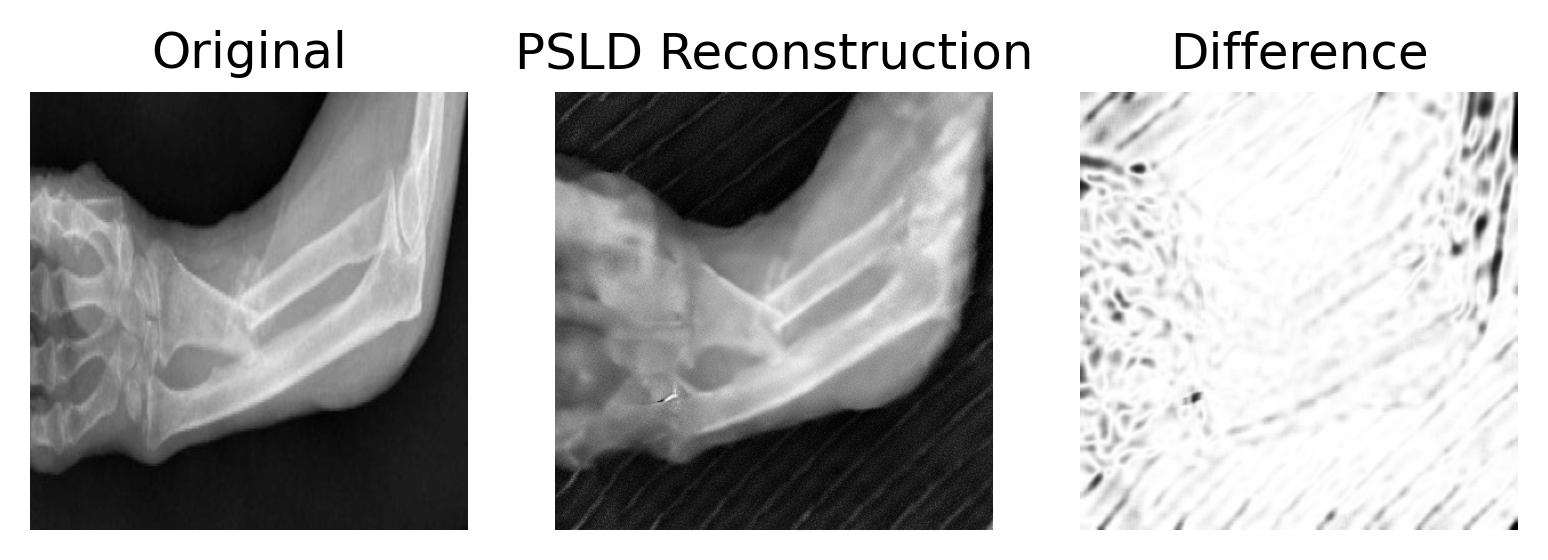
\includegraphics[width=\columnwidth]{difference.png}}
        \caption{Difference between original image and its synthetic sample. Pixel difference $x$ is scaled to $x^{400}$.}
        \label{difference}
    \end{center}
    \vskip -0.3in
\end{figure}

\section{Discussion and Future Work}

Treating data augmentation as an inverse problem allows for better variation of synthetic samples compared to naive data augmentation techniques, and can be done
without the need to retrain on a specific dataset. However as seen, the realism of the generated images are not as comparable to GANs or other diffusion based techniques,
but are inherently more faithful to the original class. Currently the PSLD algorithm is unable to effectively use the prompt as a guide to reconstruction, however if the 
affect of the prompt is consider within the gradient updates of PSLD, the potential for it's implementation could be explored. Furthermore finetuning the diffusion model on
the training set using methods such as ambient diffusion \cite{2305.19256} could also be explored in order to improve the ability of the diffusion model to generalize to 
a specific domain, i.e. medical imaging. Furthermore, an understanding into the effects that ambient diffusion has on the size of data needed to finetune diffusion models
would be interesting to explore. This could be taken a step farther by using approaches described by \cite{2302.07944}, where embeddings could be learned through
textual inversion and allow better class specific guidance through the inpainting process. 

Finally the use of other inverse problems such as motion blurring, gaussian blurring, and lossy compression could also be explored as ways to induce other types of variation
within the diffusion model. The use of inpainting is intuitive, however there is no reason to believe that other inverse problems could be used to create unique synthetic
sample reconstructions compared to other domains. 

Importantly the need to test the effectiveness of these methods for OOD datasets from diffusion models training sets is necessary in order to understand the generalizablity 
of these methods. While the use of these diffusion models is promising, the need to ensure their ability to generalize to new domains is important in understanding their ability
to create synthetic data. Further understanding of wether diffusion models are creative or have simple memorized their training set is essential to understanding their abilities,
as synthetic data generators.

% Acknowledgements should only appear in the accepted version.
\section*{Acknowledgements}

We would like to thank Litu Rout for spending time to help explain his work on solving inverse problems with PSLD. We would also like the thank the Machine Learning Lab for
providing credits in order to run our experiments.

% In the unusual situation where you want a paper to appear in the
% references without citing it in the main text, use \nocite
\bibliography{main}
\bibliographystyle{icml2021}

\end{document}


% This document was modified from the file originally made available by
% Pat Langley and Andrea Danyluk for ICML-2K. This version was created
% by Iain Murray in 2018, and modified by Alexandre Bouchard in
% 2019 and 2021. Previous contributors include Dan Roy, Lise Getoor and Tobias
% Scheffer, which was slightly modified from the 2010 version by
% Thorsten Joachims & Johannes Fuernkranz, slightly modified from the
% 2009 version by Kiri Wagstaff and Sam Roweis's 2008 version, which is
% slightly modified from Prasad Tadepalli's 2007 version which is a
% lightly changed version of the previous year's version by Andrew
% Moore, which was in turn edited from those of Kristian Kersting and
% Codrina Lauth. Alex Smola contributed to the algorithmic style files.
